\documentclass[12pt, a4paper]{article}

%% ── Geometry ────────────────────────────────────────────────────────────────
\usepackage[a4paper, top=2.5cm, bottom=2.5cm,
            left=2.8cm, right=2.8cm, headheight=15pt]{geometry}

%% ── Fonts & encoding ────────────────────────────────────────────────────────
\usepackage[T1]{fontenc}
\usepackage[utf8]{inputenc}
\usepackage{palatino}
\usepackage{mathpazo}
\usepackage{microtype}

%% ── Mathematics ─────────────────────────────────────────────────────────────
\usepackage{amsmath, amssymb, amsthm, mathtools}
\usepackage{cancel}

%% ── Graphics & colour ───────────────────────────────────────────────────────
\usepackage{xcolor}
\usepackage{tikz}
\usetikzlibrary{arrows.meta, positioning, calc,
                decorations.pathreplacing, backgrounds, patterns}
\usepackage{pgfplots}
\pgfplotsset{compat=1.15}

%% ── Tables ──────────────────────────────────────────────────────────────────
\usepackage{booktabs, array, colortbl, multirow, tabularx}
\renewcommand{\arraystretch}{1.45}

%% ── Lists ───────────────────────────────────────────────────────────────────
\usepackage{enumitem}
\setlist[itemize]{leftmargin=1.8em, itemsep=3pt, topsep=4pt}
\setlist[enumerate]{leftmargin=1.8em, itemsep=3pt, topsep=4pt}

%% ── Callout boxes ───────────────────────────────────────────────────────────
\usepackage[most]{tcolorbox}
\tcbuselibrary{skins, breakable, theorems}

%% ── Headers, footers, TOC ───────────────────────────────────────────────────
\usepackage{fancyhdr}
\usepackage{lastpage}
\usepackage{tocloft}
\usepackage{caption}

%% ── Misc ────────────────────────────────────────────────────────────────────
\usepackage{parskip}
\setlength{\parskip}{6pt}
\setlength{\parindent}{0pt}
\usepackage{float}
\usepackage[colorlinks=true, linkcolor=navy, urlcolor=navy,
            citecolor=navy]{hyperref}

%% ═══════════════════════════════════════════════════════════════════════════
%%  COLOUR PALETTE  (navy / gold / teal / crimson)
%% ═══════════════════════════════════════════════════════════════════════════
\definecolor{navy}{RGB}{10, 40, 100}
\definecolor{navylight}{RGB}{232, 238, 252}
\definecolor{gold}{RGB}{180, 130, 10}
\definecolor{lightgold}{RGB}{254, 248, 220}
\definecolor{teal}{RGB}{10, 110, 100}
\definecolor{lightteal}{RGB}{224, 248, 244}
\definecolor{crimson}{RGB}{150, 20, 30}
\definecolor{lightcrimson}{RGB}{255, 236, 236}
\definecolor{purple}{RGB}{80, 30, 130}
\definecolor{lightpurple}{RGB}{245, 238, 255}
\definecolor{solgreen}{RGB}{10, 95, 50}
\definecolor{lightsol}{RGB}{228, 252, 238}
\definecolor{charcoal}{RGB}{38, 38, 38}
\definecolor{slate}{RGB}{75, 85, 100}
\definecolor{tabhead}{RGB}{10, 40, 100}
\definecolor{tabeven}{RGB}{232, 238, 252}

%% ═══════════════════════════════════════════════════════════════════════════
%%  TCOLORBOX STYLES
%% ═══════════════════════════════════════════════════════════════════════════

\newtcolorbox{defbox}[1]{
  breakable, enhanced,
  colback=navylight, colframe=navy, coltitle=white,
  fonttitle=\bfseries\sffamily, title={Definition --- #1},
  arc=4pt, boxrule=1pt, left=8pt, right=8pt, top=6pt, bottom=6pt,
  attach boxed title to top left={yshift=-2mm, xshift=6mm},
  boxed title style={colback=navy, arc=3pt, boxrule=0pt}}

\newtcolorbox{thmbox}[1]{
  breakable, enhanced,
  colback=lightteal, colframe=teal, coltitle=white,
  fonttitle=\bfseries\sffamily, title={Theorem --- #1},
  arc=4pt, boxrule=1pt, left=8pt, right=8pt, top=6pt, bottom=6pt,
  attach boxed title to top left={yshift=-2mm, xshift=6mm},
  boxed title style={colback=teal, arc=3pt, boxrule=0pt}}

\newtcolorbox{propbox}[1]{
  breakable, enhanced,
  colback=lightteal, colframe=teal, coltitle=white,
  fonttitle=\bfseries\sffamily, title={Proposition --- #1},
  arc=4pt, boxrule=1pt, left=8pt, right=8pt, top=6pt, bottom=6pt,
  attach boxed title to top left={yshift=-2mm, xshift=6mm},
  boxed title style={colback=teal, arc=3pt, boxrule=0pt}}

\newtcolorbox{keybox}[1]{
  breakable, enhanced,
  colback=lightgold, colframe=gold, coltitle=white,
  fonttitle=\bfseries\sffamily, title={#1},
  arc=4pt, boxrule=1pt, left=8pt, right=8pt, top=6pt, bottom=6pt,
  attach boxed title to top left={yshift=-2mm, xshift=6mm},
  boxed title style={colback=gold, arc=3pt, boxrule=0pt}}

\newtcolorbox{exbox}[1]{
  breakable, enhanced,
  colback=lightpurple, colframe=purple, coltitle=white,
  fonttitle=\bfseries\sffamily, title={Worked Example --- #1},
  arc=4pt, boxrule=1pt, left=8pt, right=8pt, top=6pt, bottom=6pt,
  attach boxed title to top left={yshift=-2mm, xshift=6mm},
  boxed title style={colback=purple, arc=3pt, boxrule=0pt}}

\newtcolorbox{warnbox}[1]{
  breakable, enhanced,
  colback=lightcrimson, colframe=crimson, coltitle=white,
  fonttitle=\bfseries\sffamily, title={#1},
  arc=4pt, boxrule=1pt, left=8pt, right=8pt, top=6pt, bottom=6pt,
  attach boxed title to top left={yshift=-2mm, xshift=6mm},
  boxed title style={colback=crimson, arc=3pt, boxrule=0pt}}

\newtcolorbox{solbox}{
  breakable, enhanced,
  colback=lightsol, colframe=solgreen, coltitle=white,
  fonttitle=\bfseries\sffamily, title={Solution},
  arc=4pt, boxrule=1pt, left=8pt, right=8pt, top=6pt, bottom=6pt,
  attach boxed title to top left={yshift=-2mm, xshift=6mm},
  boxed title style={colback=solgreen, arc=3pt, boxrule=0pt}}

%% ═══════════════════════════════════════════════════════════════════════════
%%  THEOREM ENVIRONMENTS
%% ═══════════════════════════════════════════════════════════════════════════
\theoremstyle{definition}
\newtheorem{remark}{Remark}[section]

%% ═══════════════════════════════════════════════════════════════════════════
%%  MATHS MACROS
%% ═══════════════════════════════════════════════════════════════════════════
\newcommand{\R}{\mathbb{R}}
\newcommand{\dx}{\,dx}
\newcommand{\dy}{\,dy}
\newcommand{\dd}[1]{\dfrac{d}{d#1}}
\newcommand{\ddd}[2]{\dfrac{d#1}{d#2}}
\newcommand{\dddd}[2]{\dfrac{d^{2}#1}{d#2^{2}}}
\newcommand{\pp}[2]{\dfrac{\partial #1}{\partial #2}}
\newcommand{\ppp}[2]{\dfrac{\partial^2 #1}{\partial #2^2}}
\newcommand{\ppmix}[3]{\dfrac{\partial^2 #1}{\partial #2\,\partial #3}}
\newcommand{\eval}[2]{\left.#1\right|_{#2}}
\newcommand{\abs}[1]{\left|#1\right|}
\newcommand{\limit}[2]{\lim_{#1 \to #2}}
\DeclareMathOperator{\sgn}{sgn}

%% ═══════════════════════════════════════════════════════════════════════════
%%  PAGE STYLE
%% ═══════════════════════════════════════════════════════════════════════════
\pagestyle{fancy}
\fancyhf{}
\fancyhead[L]{\textcolor{navy}{\textbf{ECON 320}}
              \textcolor{slate}{ --- Comparative Statics \& Derivatives}}
\fancyhead[R]{\textcolor{slate}{\small Chiang \& Wainwright (2005)}}
\fancyfoot[C]{\textcolor{slate}{\small Page \thepage\ of \pageref{LastPage}}}
\renewcommand{\headrulewidth}{1.2pt}
\renewcommand{\headrule}{%
  \hbox to\headwidth{\color{navy}\leaders\hrule height\headrulewidth\hfill}}
\renewcommand{\footrulewidth}{0.4pt}

%% TOC
\renewcommand{\cftsecfont}{\bfseries\color{navy}}
\renewcommand{\cftsecpagefont}{\bfseries\color{navy}}
\renewcommand{\cftsubsecfont}{\color{charcoal}}
\setlength{\cftbeforesecskip}{4pt}

%% ═══════════════════════════════════════════════════════════════════════════
\begin{document}
%% ═══════════════════════════════════════════════════════════════════════════

%% ── COVER ────────────────────────────────────────────────────────────────
\thispagestyle{empty}
\begin{tikzpicture}[remember picture, overlay]
  \fill[navy] (current page.north west)
    rectangle ([yshift=-6cm] current page.north east);
  \fill[gold] ([yshift=-6cm]  current page.north west)
    rectangle ([yshift=-6.45cm] current page.north east);
\end{tikzpicture}

\vspace*{-1.6cm}
\begin{center}
  {\color{white}\large\bfseries\sffamily ECON 320 --- LECTURE NOTES}\\[10pt]
  {\color{white}\Huge\bfseries Comparative Statics and}\\[6pt]
  {\color{white}\Huge\bfseries the Concept of Derivative}\\[10pt]
  {\color{gold}\large\itshape
    Based on Chiang \& Wainwright (2005), Chapters 6--8}
\end{center}

\vspace{3.6cm}
\begin{center}
\begin{tabular}{r l}
  \textbf{\textcolor{navy}{Course}}         & ECON 320: Introduction to Mathematical Economics \\[3pt]
  \textbf{\textcolor{navy}{Primary Text}}   & A.\ C.\ Chiang \& K.\ Wainwright,
                                              \textit{Fundamental Methods of Mathematical}\\
                                            & \textit{Economics}, 4th ed., McGraw-Hill, 2005. \\[3pt]
  \textbf{\textcolor{navy}{Supplementary}}  & Hoy et al., \textit{Mathematics for Economics},
                                              3rd ed., MIT Press, 2011. \\[2pt]
                                            & Simon \& Blume, \textit{Mathematics for Economists},
                                              Norton, 1994. \\[3pt]
  \textbf{\textcolor{navy}{Topics}}         & Comparative statics, limits, derivatives,
                                              differentiation rules,\\
                                            & higher-order derivatives, partial derivatives,
                                              implicit functions \\[3pt]
  \textbf{\textcolor{navy}{Term}}           & Fall 2026 \\
\end{tabular}
\end{center}

\newpage
\tableofcontents
\newpage

%% ═══════════════════════════════════════════════════════════════════════════
\section{The Nature of Comparative Statics}
%% ═══════════════════════════════════════════════════════════════════════════

\subsection{What is Comparative Statics?}

Comparative statics is one of the most fundamental tools of economic analysis.
It asks: \textit{if an exogenous parameter of a model changes, how does the
endogenous (equilibrium) variable respond?}  We compare two static equilibria
--- the ``before'' and ``after'' --- without modelling the dynamic path between
them.
\medskip

The method permeates every field of economics:
\begin{itemize}
  \item How does equilibrium price change when a tax is imposed?
  \item How does a firm's optimal output change when input prices rise?
  \item How does the IS--LM equilibrium shift when the money supply expands?
\end{itemize}

Formally, an economic model typically specifies a system of equations in
endogenous variables $y$ and exogenous parameters $\alpha$.  Solving yields
an equilibrium $y^* = f(\alpha)$.  Comparative statics studies $dy^*/d\alpha$.

\begin{defbox}{Comparative Statics}
\textbf{Comparative statics} is the analysis of how the equilibrium value of
an endogenous variable $y^*$ changes in response to a change in an exogenous
parameter $\alpha$, holding all other exogenous variables fixed.  The central
object is the \emph{comparative-static derivative}
\[
  \ddd{y^*}{\alpha}
\]
and its sign (direction) and magnitude (size).
\end{defbox}

\subsection{A Simple Market Model}

Consider the standard competitive market.  Demand and supply are functions of
price $P$ and an exogenous shift parameter $\alpha$ (e.g.\ consumer income):
\[
  Q^d = D(P,\,\alpha), \qquad Q^s = S(P)
\]
Equilibrium requires $Q^d = Q^s$, i.e.\
\begin{equation}
  D(P^*,\,\alpha) - S(P^*) = 0
  \label{eq:eq_cond}
\end{equation}

The equilibrium price $P^*$ is implicitly a function of $\alpha$.  To find
$dP^*/d\alpha$, we differentiate \eqref{eq:eq_cond} with respect to $\alpha$
(treating $P^*$ as a function of $\alpha$):
\[
  \pp{D}{P}\ddd{P^*}{\alpha} + \pp{D}{\alpha}
  - \ddd{S}{P}\ddd{P^*}{\alpha} = 0
\]
Solving:
\begin{equation}
  \ddd{P^*}{\alpha}
  = \frac{-\,\partial D/\partial\alpha}
         {\partial D/\partial P - \partial S/\partial P}
  \label{eq:comp_stat}
\end{equation}

\begin{exbox}{Market for a Normal Good}
Let $D(P,\alpha) = a - bP + \alpha$ (linear demand, $\alpha$ = income) and
$S(P) = c + dP$.

Equilibrium: $a - bP^* + \alpha = c + dP^*$, giving
$P^* = \dfrac{a - c + \alpha}{b + d}$.

Direct differentiation:
\[
  \ddd{P^*}{\alpha} = \frac{1}{b+d} > 0
\]
since $b,d>0$.  A rise in consumer income shifts demand right and raises
equilibrium price.  Using formula \eqref{eq:comp_stat}:
$\partial D/\partial\alpha = 1$, $\partial D/\partial P = -b$,
$\partial S/\partial P = d$, so
\[
  \ddd{P^*}{\alpha} = \frac{-1}{-b - d} = \frac{1}{b+d} > 0. \quad\checkmark
\]
Comparative-static derivative for quantity:
$Q^* = c + dP^* = c + \dfrac{d(a-c+\alpha)}{b+d}$, so
$\dfrac{dQ^*}{d\alpha} = \dfrac{d}{b+d} > 0$.
Both price and quantity rise when income increases.
\end{exbox}

\subsection{The Role of the Derivative}

Comparative statics is therefore inseparable from the concept of the derivative.
The derivative of $y^* = f(\alpha)$ measures the \emph{instantaneous rate of
change} of equilibrium with respect to the parameter --- exactly what we need.
The rest of this module builds the formal theory of derivatives that makes
comparative-static analysis rigorous.

%% ═══════════════════════════════════════════════════════════════════════════
\section{The Concept of Limit}
%% ═══════════════════════════════════════════════════════════════════════════

\subsection{Rates of Change and the Difference Quotient}

Before defining the derivative, we must understand the \emph{rate of change}
of a function over a finite interval and then let that interval shrink to zero.

Let $y = f(x)$.  Suppose $x$ changes from $x_0$ to $x_0 + \Delta x$ (where
$\Delta x \neq 0$).  The corresponding change in $y$ is
$\Delta y = f(x_0 + \Delta x) - f(x_0)$.

\begin{defbox}{Difference Quotient}
The \textbf{difference quotient} (or average rate of change) of $f$ over the
interval $[x_0,\, x_0+\Delta x]$ is:
\[
  \frac{\Delta y}{\Delta x}
  = \frac{f(x_0 + \Delta x) - f(x_0)}{\Delta x}
\]
Geometrically, this is the slope of the \emph{secant line} through the points
$(x_0, f(x_0))$ and $(x_0+\Delta x,\, f(x_0+\Delta x))$.
\end{defbox}

\begin{exbox}{Difference Quotient for a Quadratic}
Let $f(x) = x^2$.  At $x_0 = 3$:
\[
  \frac{\Delta y}{\Delta x}
  = \frac{(3+\Delta x)^2 - 3^2}{\Delta x}
  = \frac{9 + 6\Delta x + (\Delta x)^2 - 9}{\Delta x}
  = 6 + \Delta x
\]
For $\Delta x = 2$: slope of secant $= 8$ (connecting $(3,9)$ and $(5,25)$).\\
For $\Delta x = 1$: slope $= 7$. \quad For $\Delta x = 0.1$: slope $= 6.1$.

As $\Delta x \to 0$, the slope approaches 6.  This will be the derivative.
\end{exbox}

\subsection{The Limit Concept}

\begin{defbox}{Limit (Informal)}
We say that $\displaystyle\limit{x}{a} f(x) = L$ if $f(x)$ can be made
arbitrarily close to $L$ by taking $x$ sufficiently close to $a$ (but
$x \neq a$).  The value of $f$ \emph{at} $a$ is irrelevant to the limit.
\end{defbox}

\begin{defbox}{Limit (Formal --- Epsilon-Delta)}
$\displaystyle\limit{x}{a} f(x) = L$ if and only if for every $\varepsilon > 0$
there exists $\delta > 0$ such that:
\[
  0 < \abs{x - a} < \delta \implies \abs{f(x) - L} < \varepsilon
\]
\end{defbox}

\begin{keybox}{Properties of Limits}
If $\displaystyle\limit{x}{a} f(x) = L$ and $\displaystyle\limit{x}{a} g(x) = M$, then:
\begin{enumerate}
  \item $\displaystyle\limit{x}{a}[f(x) + g(x)] = L + M$
  \item $\displaystyle\limit{x}{a}[f(x) \cdot g(x)] = L \cdot M$
  \item $\displaystyle\limit{x}{a}\dfrac{f(x)}{g(x)} = \dfrac{L}{M}$, provided $M \neq 0$
  \item $\displaystyle\limit{x}{a}[c \cdot f(x)] = c \cdot L$ for any constant $c$
  \item $\displaystyle\limit{x}{a}[f(x)]^n = L^n$ for positive integer $n$
\end{enumerate}
These follow directly from the epsilon-delta definition
(\textit{Chiang \& Wainwright}, p.\ 127; \textit{Simon \& Blume}, Ch.\ 2).
\end{keybox}

\begin{exbox}{Computing Limits}
\begin{enumerate}
  \item $\displaystyle\limit{x}{2}(3x^2 - 5x + 1) = 3(4) - 5(2) + 1 = 3$ \quad
    (polynomial, substitute directly)

  \item $\displaystyle\limit{x}{3}\frac{x^2-9}{x-3}$: substituting $x=3$ gives $0/0$ (indeterminate).
  Factor: $\dfrac{x^2-9}{x-3} = \dfrac{(x-3)(x+3)}{x-3} = x+3$ for $x\neq 3$.
  Therefore the limit $= 3+3 = 6$.

  \item $\displaystyle\limit{\Delta x}{0}\frac{(x+\Delta x)^2 - x^2}{\Delta x}
    = \limit{\Delta x}{0}(2x + \Delta x) = 2x$. \quad
    (This is the derivative of $x^2$.)
\end{enumerate}
\end{exbox}

\subsection{One-Sided Limits and Continuity}

\begin{defbox}{One-Sided Limits}
The \textbf{right-hand limit} is $\displaystyle\limit{x}{a^+}f(x) = L_R$
(approaching $a$ from above).\\
The \textbf{left-hand limit} is $\displaystyle\limit{x}{a^-}f(x) = L_L$
(approaching $a$ from below).\\
The (two-sided) limit exists if and only if $L_R = L_L$.
\end{defbox}

\begin{defbox}{Continuity}
$f$ is \textbf{continuous at} $x = a$ if:
\begin{enumerate}[label=(\roman*)]
  \item $f(a)$ is defined,
  \item $\displaystyle\limit{x}{a}f(x)$ exists,
  \item $\displaystyle\limit{x}{a}f(x) = f(a)$.
\end{enumerate}
$f$ is \textbf{continuous on an interval} if it is continuous at every point of
that interval.
\end{defbox}

\begin{warnbox}{Continuity Does Not Imply Differentiability}
A function can be continuous everywhere but differentiable nowhere (Weierstrass
function).  More relevantly in economics: $f(x) = |x|$ is continuous at $x=0$
but not differentiable there (the left- and right-hand derivatives differ).
However, differentiability \emph{does} imply continuity --- see Theorem~\ref{thm:diff_cont}.
\end{warnbox}

%% ═══════════════════════════════════════════════════════════════════════════
\section{The Derivative}
%% ═══════════════════════════════════════════════════════════════════════════

\subsection{Definition of the Derivative}

\begin{defbox}{The Derivative}
The \textbf{derivative} of $f$ at $x_0$, written $f'(x_0)$ or
$\left.\dfrac{dy}{dx}\right|_{x=x_0}$, is defined as:
\[
  f'(x_0)
  = \limit{\Delta x}{0} \frac{f(x_0+\Delta x) - f(x_0)}{\Delta x}
  = \limit{h}{0} \frac{f(x_0+h) - f(x_0)}{h}
\]
provided this limit exists.  When it does, $f$ is said to be
\textbf{differentiable at} $x_0$.

The \textbf{derivative function} $f': \text{domain}(f) \to \R$ assigns to
each $x$ in the domain (where the limit exists) the value $f'(x)$.
\end{defbox}

\textbf{Geometric interpretation.}  As $\Delta x \to 0$, the secant line through
$(x_0, f(x_0))$ and $(x_0+\Delta x, f(x_0+\Delta x))$ rotates toward the
\emph{tangent line} at $(x_0, f(x_0))$.  The derivative $f'(x_0)$ is the slope
of this tangent line.

\medskip

\begin{center}
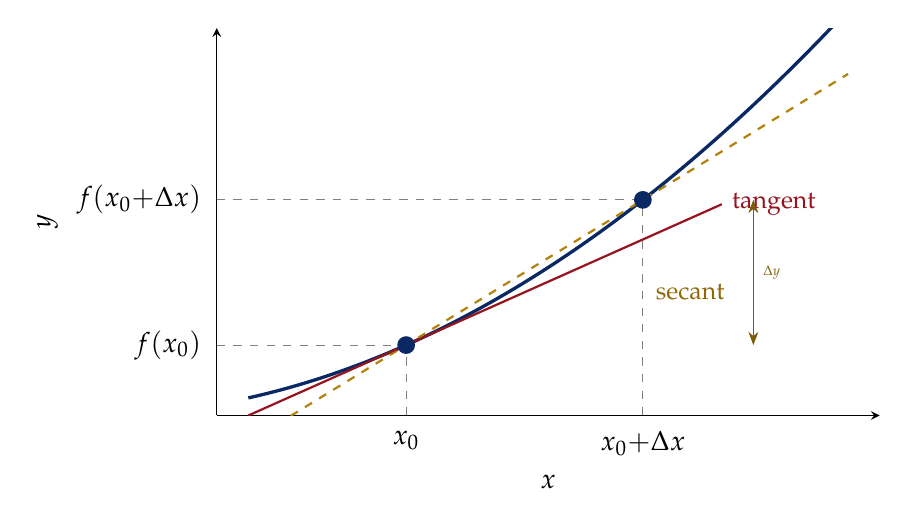
\begin{tikzpicture}
\begin{axis}[
  width=10cm, height=6.5cm,
  axis lines=left,
  xlabel={$x$}, ylabel={$y$},
  xmin=0.8, xmax=5,
  ymin=0, ymax=22,
  xtick={2,3.5},
  xticklabels={$x_0$, $x_0{+}\Delta x$},
  ytick={4,12.25},
  yticklabels={$f(x_0)$, $f(x_0{+}\Delta x)$},
  grid=none,
  tick style={draw=none},
  every axis plot/.append style={thick},
]
  %% Parabola f(x)=x^2
  \addplot[navy, very thick, domain=1:5, samples=100]{x^2}
    node[right, pos=0.95, font=\small]{$y=f(x)$};

  %% Secant line through (2,4) and (3.5,12.25): slope=(12.25-4)/1.5=5.5
  \addplot[gold, thick, dashed, domain=1:4.8]{5.5*(x-2)+4};

  %% Tangent at x=2: slope=2*2=4
  \addplot[crimson, thick, domain=1:4]{4*(x-2)+4}
    node[right, pos=1, font=\small, crimson]{tangent};

  %% Points
  \addplot[only marks, mark=*, mark size=2.8pt, navy]
    coordinates {(2,4)(3.5,12.25)};

  %% Dashed drop lines
  \addplot[gray, thin, dashed] coordinates {(2,0)(2,4)};
  \addplot[gray, thin, dashed] coordinates {(3.5,0)(3.5,12.25)};
  \addplot[gray, thin, dashed] coordinates {(0.8,4)(2,4)};
  \addplot[gray, thin, dashed] coordinates {(0.8,12.25)(3.5,12.25)};

  %% Delta x brace
  \draw[{Stealth}-{Stealth}, gold!70!black]
    (axis cs:2,-1.5) -- (axis cs:3.5,-1.5)
    node[midway, below, font=\tiny]{$\Delta x$};
  \draw[{Stealth}-{Stealth}, gold!70!black]
    (axis cs:4.2,4) -- (axis cs:4.2,12.25)
    node[midway, right, font=\tiny]{$\Delta y$};

  \node[gold!80!black, font=\small] at (axis cs:3.8,7){secant};
\end{axis}
\end{tikzpicture}
\captionof*{figure}{\small As $\Delta x\to 0$ the secant (gold) approaches the
tangent (crimson); the derivative is the slope of the tangent.}
\end{center}

\subsection{Differentiability and Continuity}

\begin{thmbox}{Differentiability Implies Continuity}
\label{thm:diff_cont}
If $f$ is differentiable at $x_0$, then $f$ is continuous at $x_0$.
\end{thmbox}

\begin{proof}
Since $f'(x_0)$ exists, write:
\[
  f(x_0+h) - f(x_0)
  = \frac{f(x_0+h)-f(x_0)}{h} \cdot h
  \xrightarrow{h\to 0} f'(x_0)\cdot 0 = 0
\]
Therefore $\displaystyle\limit{h}{0}f(x_0+h) = f(x_0)$, i.e.\ $f$ is continuous at $x_0$.
\end{proof}

\begin{exbox}{Deriving Derivatives from First Principles}

\textbf{1.} $f(x) = c$ (constant function):
\[
  f'(x) = \limit{h}{0}\frac{c - c}{h} = \limit{h}{0}0 = 0
\]

\textbf{2.} $f(x) = x^n$ for $n \in \mathbb{N}$:
\[
  f'(x)
  = \limit{h}{0}\frac{(x+h)^n - x^n}{h}
\]
By the Binomial Theorem:
$(x+h)^n = x^n + nx^{n-1}h + \binom{n}{2}x^{n-2}h^2 + \cdots + h^n$

\[
  f'(x) = \limit{h}{0}\frac{nx^{n-1}h + \binom{n}{2}x^{n-2}h^2 + \cdots}{h}
         = \limit{h}{0}\left[nx^{n-1} + \binom{n}{2}x^{n-2}h + \cdots\right]
         = nx^{n-1}
\]

\textbf{3.} $f(x) = \sqrt{x}$ for $x > 0$:
\[
  f'(x) = \limit{h}{0}\frac{\sqrt{x+h}-\sqrt{x}}{h}
         = \limit{h}{0}\frac{(\sqrt{x+h}-\sqrt{x})(\sqrt{x+h}+\sqrt{x})}
                            {h(\sqrt{x+h}+\sqrt{x})}
         = \limit{h}{0}\frac{1}{\sqrt{x+h}+\sqrt{x}}
         = \frac{1}{2\sqrt{x}}
\]

\textbf{4.} $f(x) = e^x$:
\[
  f'(x) = \limit{h}{0}\frac{e^{x+h}-e^x}{h}
         = e^x\limit{h}{0}\frac{e^h-1}{h} = e^x \cdot 1 = e^x
\]
(using the standard result $\lim_{h\to 0}(e^h-1)/h = 1$).
\end{exbox}

\subsection{Notation}

There are several equivalent notations for the derivative
(\textit{Chiang \& Wainwright}, p.\ 132):
\[
  f'(x) \;=\; \ddd{y}{x} \;=\; \ddd{f}{x} \;=\; \dot y \;=\; Df(x) \;=\; y'
\]
The Leibniz notation $dy/dx$ is especially useful in economics because it
reminds us of the units (change in $y$ per unit change in $x$) and is
convenient for the chain rule.

%% ═══════════════════════════════════════════════════════════════════════════
\section{Rules of Differentiation}
%% ═══════════════════════════════════════════════════════════════════════════

\subsection{Basic Rules}

The following rules allow us to differentiate any combination of elementary
functions without returning to the first-principles limit definition.  All are
proved using limit properties.

\begin{thmbox}{Basic Differentiation Rules}
Let $f$ and $g$ be differentiable at $x$, and $c \in \R$ a constant.
\begin{enumerate}
  \item \textbf{Constant Rule}: $\dd{x}[c] = 0$
  \item \textbf{Power Rule}: $\dd{x}[x^n] = nx^{n-1}$ for any $n \in \R$
  \item \textbf{Constant Multiple}: $\dd{x}[c\,f(x)] = c\,f'(x)$
  \item \textbf{Sum/Difference}: $\dd{x}[f(x)\pm g(x)] = f'(x)\pm g'(x)$
  \item \textbf{Product Rule}: $\dd{x}[f(x)\,g(x)] = f'(x)\,g(x) + f(x)\,g'(x)$
  \item \textbf{Quotient Rule}:
    $\dd{x}\!\left[\dfrac{f(x)}{g(x)}\right]
    = \dfrac{f'(x)\,g(x) - f(x)\,g'(x)}{[g(x)]^2}$, \; $g(x)\neq 0$
  \item \textbf{Chain Rule}: If $y = f(u)$ and $u = g(x)$, then
    $\ddd{y}{x} = \ddd{y}{u}\cdot\ddd{u}{x} = f'(g(x))\cdot g'(x)$
\end{enumerate}
\end{thmbox}

\begin{exbox}{Applying the Basic Rules}
\textbf{1. Power and Sum:} $f(x) = 4x^3 - 7x^2 + 2x - 9$
\[
  f'(x) = 4(3x^2) - 7(2x) + 2(1) - 0 = 12x^2 - 14x + 2
\]

\textbf{2. Product Rule:} $f(x) = (2x^2+1)(x^3-3x)$

Let $u = 2x^2+1$, $v = x^3-3x$, so $u'=4x$, $v'=3x^2-3$.
\[
  f'(x) = (4x)(x^3-3x) + (2x^2+1)(3x^2-3)
        = 4x^4 - 12x^2 + 6x^4 - 6x^2 + 3x^2 - 3
        = 10x^4 - 15x^2 - 3
\]

\textbf{3. Quotient Rule:} $f(x) = \dfrac{x^2+1}{x-1}$, $x\neq 1$
\[
  f'(x) = \frac{2x(x-1) - (x^2+1)(1)}{(x-1)^2}
        = \frac{2x^2-2x-x^2-1}{(x-1)^2}
        = \frac{x^2-2x-1}{(x-1)^2}
\]

\textbf{4. Chain Rule:} $f(x) = (3x^2+5)^7$

Let $u = 3x^2+5$, $y = u^7$. Then $dy/du = 7u^6$, $du/dx = 6x$.
\[
  f'(x) = 7(3x^2+5)^6 \cdot 6x = 42x(3x^2+5)^6
\]
\end{exbox}

\subsection{Derivatives of Exponential and Logarithmic Functions}

\begin{keybox}{Standard Results for Exp and Log}
\begin{align*}
  \dd{x}[e^x] &= e^x \\[4pt]
  \dd{x}[e^{ax}] &= a\,e^{ax} \qquad (a\in\R) \\[4pt]
  \dd{x}[a^x] &= a^x\ln a \qquad (a>0,\;a\neq 1)\\[4pt]
  \dd{x}[\ln x] &= \frac{1}{x} \qquad (x>0) \\[4pt]
  \dd{x}[\ln|x|] &= \frac{1}{x} \qquad (x\neq 0) \\[4pt]
  \dd{x}[\log_a x] &= \frac{1}{x\ln a} \qquad (a>0,\;a\neq 1,\;x>0)
\end{align*}
\end{keybox}

\begin{exbox}{Exponential and Log Derivatives in Economics}
\textbf{1. Continuous compounding.}  Value of an investment:
$V(t) = V_0 e^{rt}$.  Rate of growth:
\[
  V'(t) = V_0\,r\,e^{rt} = r\,V(t)
\]
The instantaneous rate of growth is $V'(t)/V(t) = r$ --- the continuous
interest rate.

\textbf{2. Log-linear demand.}
$\ln Q = a - b\ln P \Rightarrow Q = e^a P^{-b}$.  The price elasticity:
\[
  \varepsilon = \ddd{\ln Q}{\ln P} = -b
\]
This is why log-linear (log-log) regressions yield constant elasticity.

\textbf{3. Chain rule with log:}
$f(x) = \ln(3x^2+1)$.  Let $u = 3x^2+1$:
\[
  f'(x) = \frac{1}{u}\cdot 6x = \frac{6x}{3x^2+1}
\]
\end{exbox}

\subsection{The Chain Rule and Composite Functions}

The chain rule is indispensable in comparative statics, where equilibrium values
depend on parameters through multiple layers of functional composition.

\begin{keybox}{Chain Rule --- Multiple Layers}
If $y = f(u)$, $u = g(v)$, $v = h(x)$, then:
\[
  \ddd{y}{x} = \ddd{y}{u}\cdot\ddd{u}{v}\cdot\ddd{v}{x}
             = f'(g(h(x)))\cdot g'(h(x))\cdot h'(x)
\]
\end{keybox}

\begin{exbox}{Chain Rule in a Macro Model}
In an IS-LM model suppose output $Y$ depends on investment $I$, investment
depends on interest rate $r$, and the interest rate depends on money supply $M$:
\[
  Y = f(I),\quad I = g(r),\quad r = h(M)
\]
The multiplier $dY/dM$ is:
\[
  \ddd{Y}{M} = \ddd{Y}{I}\cdot\ddd{I}{r}\cdot\ddd{r}{M}
             = f'(I)\cdot g'(r)\cdot h'(M)
\]
If $f'>0$ (higher investment raises output), $g'<0$ (investment falls when
interest rises), and $h'<0$ (higher money supply lowers interest rate), then:
$dY/dM = (+)(-)(-) > 0$: monetary expansion raises output.
\end{exbox}

\subsection{The Inverse Function Rule}

\begin{thmbox}{Inverse Function Rule}
If $y = f(x)$ is strictly monotone and differentiable with $f'(x) \neq 0$,
then its inverse function $x = f^{-1}(y)$ is differentiable and:
\[
  \ddd{x}{y} = \frac{1}{\,dy/dx\,} = \frac{1}{f'(x)}
\]
\end{thmbox}

\begin{exbox}{Inverse Demand and Supply}
\textbf{Demand:} $Q = 100 - 2P$.  Then $\dfrac{dQ}{dP} = -2$.

Inverse demand: $P = 50 - Q/2$, so $\dfrac{dP}{dQ} = -\dfrac{1}{2}$.

Check: $\dfrac{dP}{dQ} = 1\big/(dQ/dP) = 1/(-2) = -1/2$. $\checkmark$

\textbf{Application --- Marginal Revenue:}
$\text{TR} = P \cdot Q = (50-Q/2)\cdot Q = 50Q - Q^2/2$.
$\text{MR} = d(\text{TR})/dQ = 50 - Q$.

The slope of MR is exactly twice the slope of inverse demand.
This is the standard result: $\text{MR} = P + Q\,(dP/dQ)$.
\end{exbox}

%% ═══════════════════════════════════════════════════════════════════════════
\section{Higher-Order Derivatives}
%% ═══════════════════════════════════════════════════════════════════════════

\subsection{Second and Higher Derivatives}

\begin{defbox}{Higher-Order Derivatives}
If $f'(x)$ is itself differentiable, its derivative is the
\textbf{second derivative}:
\[
  f''(x) = \dddd{y}{x} = \ddd{}{x}\!\left[\ddd{y}{x}\right]
         = D^2 f(x) = y''
\]
The $n$-th derivative is defined recursively:
$f^{(n)}(x) = \ddd{}{x}[f^{(n-1)}(x)]$.
\end{defbox}

\textbf{Economic interpretations:}
\begin{itemize}
  \item If $y(t)$ is position at time $t$: $y'(t)$ is velocity,
    $y''(t)$ is acceleration.
  \item If $f(x)$ is a cost function: $f'(x) = \text{MC}$ (marginal cost),
    $f''(x)$ measures the rate of change of MC.
  \item If $f''(x) > 0$ at a critical point, we have a local minimum
    (second-order condition for minimisation).
  \item If $f''(x) < 0$ at a critical point, we have a local maximum
    (SOC for maximisation).
\end{itemize}

\begin{exbox}{Higher Derivatives and Diminishing Returns}
Production function: $Q = f(L) = 10L^{0.5}$ (square-root technology).

\[
  f'(L) = 5L^{-0.5} = \frac{5}{\sqrt{L}} > 0
  \quad\text{(positive marginal product)}
\]
\[
  f''(L) = -\frac{5}{2}L^{-3/2} < 0
  \quad\text{(diminishing marginal product)}
\]

The negative second derivative captures the law of diminishing returns:
each additional unit of labour adds less to output than the previous unit.

Third derivative: $f'''(L) = \frac{15}{4}L^{-5/2} > 0$ --- the rate of
diminution is itself decreasing (marginal product falls at a decreasing rate).
\end{exbox}

\subsection{Concavity, Convexity, and Inflection Points}

\begin{defbox}{Concavity and Convexity}
Let $f$ be twice differentiable on an interval $I$.
\begin{itemize}
  \item $f$ is \textbf{strictly concave} on $I$ if $f''(x) < 0$ for all $x \in I$.
  \item $f$ is \textbf{strictly convex} on $I$ if $f''(x) > 0$ for all $x \in I$.
\end{itemize}
An \textbf{inflection point} is a point where $f''$ changes sign
(concavity reverses); necessarily $f''(x_0) = 0$ there.
\end{defbox}

\begin{exbox}{Cubic Cost Function}
Total cost: $C(Q) = Q^3 - 6Q^2 + 15Q + 10$.
\[
  C'(Q) = 3Q^2 - 12Q + 15 \quad\text{(MC)}
\]
\[
  C''(Q) = 6Q - 12 \quad\text{(slope of MC)}
\]

$C''(Q) = 0 \Rightarrow Q = 2$.

For $Q < 2$: $C'' < 0$ (MC is falling --- economies of scale).\\
For $Q > 2$: $C'' > 0$ (MC is rising --- diseconomies of scale).

$Q = 2$ is the inflection point of $C$ and the minimum of MC, corresponding
to the \emph{minimum efficient scale}.
\end{exbox}

%% ═══════════════════════════════════════════════════════════════════════════
\section{Optimisation: First- and Second-Order Conditions}
%% ═══════════════════════════════════════════════════════════════════════════

\subsection{Unconstrained Optimisation in One Variable}

\begin{thmbox}{First- and Second-Order Conditions}
Let $f$ be twice differentiable on an open interval.

\textbf{First-Order Condition (FOC):} A necessary condition for $x^*$ to be
a local maximum or minimum is:
\[
  f'(x^*) = 0 \qquad (\text{critical point})
\]

\textbf{Second-Order Condition (SOC):}
\begin{itemize}
  \item If $f'(x^*) = 0$ and $f''(x^*) < 0$: $x^*$ is a \textbf{local maximum}.
  \item If $f'(x^*) = 0$ and $f''(x^*) > 0$: $x^*$ is a \textbf{local minimum}.
  \item If $f'(x^*) = 0$ and $f''(x^*) = 0$: \emph{inconclusive} --- examine
    higher derivatives or use other methods.
\end{itemize}
\end{thmbox}

\begin{exbox}{Monopoly Profit Maximisation}
Inverse demand: $P = 100 - Q$.
Total cost: $C(Q) = Q^2 + 20Q + 50$.

\textbf{Profit function:}
$\pi(Q) = (100-Q)Q - (Q^2+20Q+50) = -2Q^2 + 80Q - 50$

\textbf{FOC:}
\[
  \pi'(Q) = -4Q + 80 = 0 \implies Q^* = 20
\]

\textbf{SOC:}
\[
  \pi''(Q) = -4 < 0 \quad\text{for all }Q
\]
Confirms $Q^* = 20$ is a (global) maximum.

\textbf{Equilibrium values:}
$P^* = 100 - 20 = 80$,\quad
$\pi^* = -2(400) + 80(20) - 50 = -800 + 1600 - 50 = 750$

\textbf{Comparative statics:} Suppose the cost function shifts ---
$C(Q) = Q^2 + 20Q + c$ where $c$ is a fixed cost.  Clearly $Q^*$ does
not depend on $c$ (fixed costs don't affect the FOC).  But if the
variable cost shifts: $C(Q) = Q^2 + \alpha Q + 50$, then
$\pi(Q) = -2Q^2 + (80-\alpha)Q - 50$,
FOC: $-4Q + (80-\alpha) = 0 \Rightarrow Q^* = (80-\alpha)/4$.
\[
  \ddd{Q^*}{\alpha} = -\frac{1}{4} < 0
\]
A rise in variable cost reduces monopoly output.
\end{exbox}

\subsection{The Envelope Theorem}

The Envelope Theorem provides an elegant shortcut for comparative statics: it
tells us how the \emph{optimal value function} changes with a parameter without
re-solving the full optimisation.

\begin{thmbox}{Envelope Theorem (One Variable)}
Let $f(x;\alpha)$ be differentiable in both $x$ and $\alpha$.  Suppose
$x^*(\alpha) = \arg\max_x f(x;\alpha)$ is interior and satisfies the FOC
$f_x(x^*;\alpha) = 0$.  Define the value function
$V(\alpha) = f(x^*(\alpha);\alpha)$.  Then:
\[
  \ddd{V}{\alpha}
  = \left.\pp{f(x;\alpha)}{\alpha}\right|_{x=x^*(\alpha)}
\]
We differentiate $f$ directly with respect to $\alpha$, holding $x$ fixed at
$x^*$, ignoring the indirect effect through $x^*(\alpha)$.
\end{thmbox}

\begin{exbox}{Envelope Theorem in Producer Theory}
A competitive firm maximises $\pi = Pf(L) - wL - rK$, where $P$ (output
price), $w$ (wage), $r$ (rental rate), and $K$ are exogenous parameters.

FOC (choosing $L$): $Pf'(L^*) = w$.

By the Envelope Theorem:
\[
  \ddd{\pi^*}{P} = \eval{\pp{\pi}{P}}{L=L^*} = f(L^*) = Q^* > 0
  \quad\text{(higher price raises profit)}
\]
\[
  \ddd{\pi^*}{w} = \eval{\pp{\pi}{w}}{L=L^*} = -L^* < 0
  \quad\text{(higher wage lowers profit)}
\]
These are \textbf{Hotelling's Lemma}: $\partial\pi^*/\partial P = Q^*$
and $\partial\pi^*/\partial w = -L^*$.
\end{exbox}

%% ═══════════════════════════════════════════════════════════════════════════
\section{Partial Derivatives}
%% ═══════════════════════════════════════════════════════════════════════════

\subsection{Definition and Interpretation}

Most economic functions depend on more than one variable.
A demand function $Q^d = D(P, P_s, P_c, Y)$ depends on own price,
substitute price, complement price, and income.  The partial derivative
measures the effect of \emph{one} variable while holding all others constant
--- the ceteris paribus condition, formalised.

\begin{defbox}{Partial Derivative}
For $z = f(x,y)$, the \textbf{partial derivative} with respect to $x$ is:
\[
  \pp{f}{x} = f_x(x,y)
  = \limit{h}{0}\frac{f(x+h,\,y) - f(x,\,y)}{h}
\]
obtained by differentiating with respect to $x$ while treating $y$ as a
constant.  Similarly, $\partial f/\partial y = f_y$ holds $x$ fixed.
\end{defbox}

\begin{exbox}{Computing Partial Derivatives}
\textbf{1.} $f(x,y) = 3x^2y + 4xy^3 - 7y^2$
\[
  f_x = 6xy + 4y^3, \qquad f_y = 3x^2 + 12xy^2 - 14y
\]

\textbf{2. Cobb-Douglas:} $Q = AK^\alpha L^\beta$
\[
  \pp{Q}{K} = \alpha AK^{\alpha-1}L^\beta
            = \alpha\frac{Q}{K} \quad\text{(marginal product of capital)}
\]
\[
  \pp{Q}{L} = \beta AK^\alpha L^{\beta-1}
            = \beta\frac{Q}{L} \quad\text{(marginal product of labour)}
\]

\textbf{3. CES utility:} $U = (x_1^\rho + x_2^\rho)^{1/\rho}$
\[
  \pp{U}{x_1}
  = \frac{1}{\rho}(x_1^\rho+x_2^\rho)^{1/\rho-1}\cdot\rho x_1^{\rho-1}
  = \left(\frac{x_1^\rho+x_2^\rho}{x_1^\rho}\right)^{(1/\rho)-1}
  = U^{1-\rho}\,x_1^{\rho-1}
\]
\end{exbox}

\subsection{Second-Order Partial Derivatives}

\begin{defbox}{Second-Order Partial Derivatives}
For $z = f(x,y)$, the four second-order partials are:
\[
  f_{xx} = \ppp{f}{x}, \quad
  f_{yy} = \ppp{f}{y}, \quad
  f_{xy} = \ppmix{f}{x}{y}, \quad
  f_{yx} = \ppmix{f}{y}{x}
\]
$f_{xy}$ and $f_{yx}$ are \textbf{cross partial derivatives}.
\end{defbox}

\begin{thmbox}{Young's Theorem (Symmetry of Cross Partials)}
If $f_{xy}$ and $f_{yx}$ are both continuous at $(x_0,y_0)$, then:
\[
  f_{xy}(x_0,y_0) = f_{yx}(x_0,y_0)
\]
\emph{The order of partial differentiation does not matter under continuity.}
(\textit{Chiang \& Wainwright}, p.\ 197; \textit{Simon \& Blume}, p.\ 336.)
\end{thmbox}

\begin{exbox}{Young's Theorem in Practice}
$f(x,y) = x^3 y^2 + e^{xy}$

$f_x = 3x^2y^2 + ye^{xy}$, \quad
$f_{xy} = 6x^2y + e^{xy} + xye^{xy} = 6x^2y + (1+xy)e^{xy}$

$f_y = 2x^3y + xe^{xy}$, \quad
$f_{yx} = 6x^2y + e^{xy} + xye^{xy} = 6x^2y + (1+xy)e^{xy}$

$f_{xy} = f_{yx}$. \checkmark
\end{exbox}

\subsection{The Total Differential}

\begin{defbox}{Total Differential}
For $z = f(x,y)$, the \textbf{total differential} is:
\[
  dz = \pp{f}{x}\,dx + \pp{f}{y}\,dy = f_x\,dx + f_y\,dy
\]
It approximates the \emph{total change} in $z$ resulting from small changes
$dx$ and $dy$ in both arguments simultaneously.

More generally, for $z = f(x_1,\ldots,x_n)$:
\[
  dz = \sum_{i=1}^n \pp{f}{x_i}\,dx_i
\]
\end{defbox}

\begin{exbox}{Total Differential in Consumer Theory}
Utility $U = f(x_1, x_2)$.  Along an indifference curve, $dU = 0$:
\[
  dU = \pp{U}{x_1}dx_1 + \pp{U}{x_2}dx_2 = 0
\]
\[
  \implies \frac{dx_2}{dx_1} = -\frac{\partial U/\partial x_1}{\partial U/\partial x_2}
                              = -\frac{MU_1}{MU_2} = -\text{MRS}_{12}
\]
The slope of the indifference curve equals the negative of the marginal rate
of substitution.  This derivation uses nothing beyond the total differential.
\end{exbox}

%% ═══════════════════════════════════════════════════════════════════════════
\section{Implicit Function Theorem}
%% ═══════════════════════════════════════════════════════════════════════════

\subsection{Implicit Differentiation}

Many economic relationships are defined implicitly --- equilibrium conditions
rather than explicit solved-out equations.  We cannot always write $y = f(x)$
explicitly, but we can still find $dy/dx$ by differentiating the implicit
equation.

\begin{thmbox}{Implicit Function Theorem (One Equation)}
Let $F(y, x) = 0$ define $y$ implicitly as a function of $x$ near
$(y_0, x_0)$.  If $F$ is continuously differentiable and $F_y \neq 0$ at
$(y_0, x_0)$, then $y = y(x)$ exists locally and:
\[
  \ddd{y}{x} = -\frac{F_x}{F_y}
\]
(\textit{Chiang \& Wainwright}, p.\ 192; \textit{Hoy et al.}, Ch.\ 14;
\textit{Simon \& Blume}, Theorem~15.7.)
\end{thmbox}

\begin{proof}[Derivation via Total Differential]
Differentiate $F(y,x) = 0$ totally:
\[
  F_y\,dy + F_x\,dx = 0
  \implies \ddd{y}{x} = -\frac{F_x}{F_y} \quad (F_y \neq 0)
\]
\end{proof}

\begin{exbox}{Market Equilibrium --- Implicit Differentiation}
Equilibrium condition: $F(P, t) = D(P) - S(P) - t = 0$

where $t$ is an excise tax (the supply curve shifts by $t$).

\[
  F_P = D'(P) - S'(P), \qquad F_t = -1
\]
\[
  \ddd{P}{t} = -\frac{F_t}{F_P} = -\frac{-1}{D'(P)-S'(P)}
             = \frac{1}{D'(P)-S'(P)}
\]

Since $D'<0$ (demand downward sloping) and $S'>0$ (supply upward sloping):
$D'(P) - S'(P) < 0$, so $\dfrac{dP}{dt} < 0$?

Wait: note the sign. $D'(P)-S'(P) < 0$, so $dP/dt = 1/(\text{negative}) < 0$?

Recheck: an excise tax shifts the supply schedule \emph{up}.  Rewrite as
$D(P)=S(P)+t$, so $F(P,t)=D(P)-S(P)-t=0$.
Tax up $\Rightarrow$ supply up $\Rightarrow$ price up.
We need: $D'(P)\,dP = S'(P)\,dP + dt \Rightarrow dP/dt = 1/(D'-S') > 0$?

Sign: $D' - S' = (\text{negative}) - (\text{positive}) < 0$, giving $dP/dt < 0$.

This contradicts intuition.  The resolution: in the standard model we write
the equilibrium as $D(P) = S(P-t)$ (tax on producers).  Then
$F = D(P) - S(P-t) = 0$, $F_P = D'-S'$, $F_t = S' > 0$, so
$dP/dt = -S'/(D'-S') \in (0,1)$ since $D'<0<S'$.

\textbf{Result:} Consumer price rises by $dP/dt = \dfrac{-S'}{D'-S'}
= \dfrac{S'}{S'-D'} \in (0,1)$.

Tax incidence on consumers: $dP/dt = S'/(S'-D')$; on producers:
$1-dP/dt = -D'/(S'-D')$.  Both shares are positive and sum to 1.
\end{exbox}

\begin{exbox}{Isoquant Slope via Implicit Differentiation}
Production function $Q = F(K,L) = \overline{Q}$ defines an isoquant
implicitly.  Setting $F(K,L) - \overline{Q} = 0 \equiv G(K,L) = 0$:
\[
  \ddd{L}{K}\bigg|_{dQ=0} = -\frac{G_K}{G_L}
  = -\frac{F_K}{F_L}
  = -\frac{MP_K}{MP_L}
  = -\text{MRTS}_{KL}
\]
The slope of the isoquant equals the negative of the Marginal Rate of
Technical Substitution --- derived purely from the implicit function rule.
\end{exbox}

\subsection{Comparative Statics with Multiple Equations}

When the model has $n$ equations and $n$ endogenous variables, matrix methods
are needed.  Differentiate the system $\mathbf{F}(\mathbf{y};\alpha) = \mathbf{0}$
totally:
\[
  \mathbf{J}\,d\mathbf{y} + \mathbf{F}_\alpha\,d\alpha = \mathbf{0}
  \quad\Rightarrow\quad
  \ddd{\mathbf{y}}{\alpha} = -\mathbf{J}^{-1}\mathbf{F}_\alpha
\]
where $\mathbf{J}$ is the Jacobian matrix of partial derivatives.

\begin{exbox}{IS-LM Comparative Statics}
The IS-LM system in two endogenous variables $(Y,r)$:
\begin{align*}
  \text{IS:} & \quad Y - C(Y) - I(r) - G = 0 \\
  \text{LM:} & \quad L(Y,r) - \frac{M}{P} = 0
\end{align*}
Total differentiation with respect to $G$ (holding $M/P$ fixed):
\[
  \begin{pmatrix}1-C'(Y) & -I'(r)\\ L_Y & L_r\end{pmatrix}
  \begin{pmatrix}dY\\ dr\end{pmatrix}
  =
  \begin{pmatrix}1 \\ 0\end{pmatrix}dG
\]
By Cramer's Rule (or matrix inversion), with $|J| = (1-C')L_r - L_Y(-I')$:
\[
  \ddd{Y}{G} = \frac{L_r}{\lvert J\rvert}, \qquad
  \ddd{r}{G} = \frac{-(L_Y)}{\lvert J\rvert}
\]
Standard sign assumptions: $0<C'<1$, $I'<0$, $L_Y>0$, $L_r<0$.

$|J| = (1-C')L_r + I'L_Y < 0 + (\text{negative}) < 0$.

$dY/dG = L_r/|J| = (\text{negative})/(\text{negative}) > 0$:
fiscal expansion raises output (IS-LM multiplier).
\end{exbox}

%% ═══════════════════════════════════════════════════════════════════════════
\section{The Concept of Elasticity}
%% ═══════════════════════════════════════════════════════════════════════════

\begin{defbox}{Point Elasticity}
The \textbf{point elasticity} of $y$ with respect to $x$ measures the
percentage change in $y$ per one-percent change in $x$:
\[
  \varepsilon_{y,x}
  = \frac{dy/y}{dx/x}
  = \ddd{y}{x}\cdot\frac{x}{y}
  = \ddd{\ln y}{\ln x}
\]
Elasticity is a \emph{unit-free} measure of responsiveness.
\end{defbox}

\begin{exbox}{Elasticities in Demand Analysis}
\textbf{1. Linear demand:} $Q = 100 - 2P$.
\[
  \varepsilon_{Q,P} = \ddd{Q}{P}\cdot\frac{P}{Q}
                    = (-2)\cdot\frac{P}{100-2P}
\]
At $P=20$: $Q=60$, $\varepsilon = (-2)(20/60) = -2/3$ (inelastic).
At $P=40$: $Q=20$, $\varepsilon = (-2)(40/20) = -4$ (elastic).

\textbf{2. Constant-elasticity demand:} $Q = AP^{-b}$.
\[
  \varepsilon_{Q,P} = -bAP^{-b-1}\cdot\frac{P}{AP^{-b}}
                    = -b \quad\text{(constant)}
\]

\textbf{3. Income elasticity of demand:}
$Q = a - bP + cY$.
\[
  \varepsilon_{Q,Y} = c\cdot\frac{Y}{Q}
\]
Normal good: $c>0$ so $\varepsilon_{Q,Y}>0$.  Luxury: $\varepsilon>1$.

\textbf{4. Output elasticity of capital (Cobb-Douglas):}
$Q = AK^\alpha L^\beta$.
\[
  \varepsilon_{Q,K} = \ddd{Q}{K}\cdot\frac{K}{Q}
                    = \alpha AK^{\alpha-1}L^\beta\cdot\frac{K}{AK^\alpha L^\beta}
                    = \alpha
\]
The output elasticity equals the capital share parameter $\alpha$.
\end{exbox}

%% ═══════════════════════════════════════════════════════════════════════════
\section{Practice Questions}
%% ═══════════════════════════════════════════════════════════════════════════

\subsection{Section A: Limits and Derivatives from First Principles}

\begin{enumerate}[label=\textbf{A\arabic*.}, leftmargin=2.5em]

\item \textbf{(First Principles)}
Use the definition $f'(x_0) = \lim_{h\to 0}\dfrac{f(x_0+h)-f(x_0)}{h}$
to find the derivative of each function at the indicated point.
\begin{enumerate}[label=(\alph*)]
  \item $f(x) = 3x^2 - 2x + 1$ at $x_0 = 2$
  \item $f(x) = 1/x$ at $x_0 = x$ (general point)
  \item $f(x) = \sqrt{x}$ at $x_0 = 4$
\end{enumerate}

\item \textbf{(Limits)}
Evaluate each limit, showing all steps.
\begin{enumerate}[label=(\alph*)]
  \item $\displaystyle\lim_{x\to 3}\frac{x^2-9}{x-3}$
  \item $\displaystyle\lim_{h\to 0}\frac{(2+h)^3-8}{h}$
  \item $\displaystyle\lim_{x\to 0}\frac{e^{3x}-1}{x}$
  \item $\displaystyle\lim_{x\to\infty}\frac{4x^2-3x}{7x^2+2}$
\end{enumerate}

\item \textbf{(Continuity)}
Determine whether each function is continuous at the indicated point.
\begin{enumerate}[label=(\alph*)]
  \item $f(x) = \dfrac{x^2-4}{x-2}$ at $x=2$
  \item $g(x) = \begin{cases} x^2 & x < 1 \\ 2x-1 & x \geq 1 \end{cases}$
        at $x=1$
  \item $h(x) = \dfrac{\sin x}{x}$ at $x = 0$ (define $h(0)=1$)
\end{enumerate}

\end{enumerate}

\subsection{Section B: Differentiation Rules}

\begin{enumerate}[label=\textbf{B\arabic*.}, leftmargin=2.5em]

\item \textbf{(Standard Rules)}
Differentiate each function with respect to $x$.
\begin{enumerate}[label=(\alph*)]
  \item $f(x) = 5x^4 - 3x^3 + 2x^2 - 7x + 11$
  \item $g(x) = (2x^3-1)(x^2+3x)$
  \item $h(x) = \dfrac{x^2-2x+1}{x^2+1}$
  \item $k(x) = e^{3x^2-1}$
  \item $\ell(x) = \ln\!\left(\dfrac{x^2+1}{x-1}\right)$, $x>1$
  \item $m(x) = x^3 e^{-2x}$
\end{enumerate}

\item \textbf{(Chain Rule)}
Differentiate using the chain rule.
\begin{enumerate}[label=(\alph*)]
  \item $y = (3x^2+2x-1)^5$
  \item $y = e^{-x^2}$
  \item $y = \ln(\ln x)$, $x>1$
  \item $y = \left(\dfrac{x+1}{x-1}\right)^3$, $x\neq 1$
\end{enumerate}

\item \textbf{(Inverse Function)}
Given $f(x) = 2x^3 + 3$, find $df^{-1}/dy$ at the point where $y=29$.

\item \textbf{(Higher-Order Derivatives)}
Find $f'$, $f''$, and $f'''$ for:
\begin{enumerate}[label=(\alph*)]
  \item $f(x) = x^5 - 4x^3 + 2x$
  \item $f(x) = xe^x$
  \item $f(x) = \ln x$, $x>0$
\end{enumerate}

\end{enumerate}

\subsection{Section C: Partial Derivatives and Total Differentials}

\begin{enumerate}[label=\textbf{C\arabic*.}, leftmargin=2.5em]

\item \textbf{(Partial Derivatives)}
For each function, compute $f_x$, $f_y$, $f_{xx}$, $f_{yy}$, and $f_{xy}$.
\begin{enumerate}[label=(\alph*)]
  \item $f(x,y) = x^3y^2 - 4x^2y + 3y^3$
  \item $f(x,y) = e^{x^2+y^2}$
  \item $f(x,y) = \ln(xy) + x^2/y$, $x,y>0$
\end{enumerate}

\item \textbf{(Total Differential)}
\begin{enumerate}[label=(\alph*)]
  \item Find $dz$ for $z = x^2y^3 - 3xy + 5y$.
  \item For the production function $Q = K^{0.4}L^{0.6}$, find the total
    differential $dQ$ and use it to approximate the change in output when $K$
    rises from 100 to 101 and $L$ rises from 64 to 65.
\end{enumerate}

\item \textbf{(Young's Theorem)}
Verify Young's Theorem for $f(x,y) = x^2 e^y + 3x\ln y$, $y>0$.

\end{enumerate}

\subsection{Section D: Comparative Statics and Implicit Differentiation}

\begin{enumerate}[label=\textbf{D\arabic*.}, leftmargin=2.5em]

\item \textbf{(Implicit Differentiation)}
\begin{enumerate}[label=(\alph*)]
  \item Find $dy/dx$ if $x^3 + y^3 = 6xy$.
  \item Find $dy/dx$ if $e^{xy} = x + y^2$.
  \item For the equilibrium condition $\alpha Q^2 - \beta Q + P = 0$
    (with $\alpha,\beta>0$), find $dQ/dP$ using the implicit function rule.
\end{enumerate}

\item \textbf{(Market Comparative Statics)}
A competitive market has:
\[
  Q^d = a - bP + cY, \quad Q^s = d + eP - fW
\]
where $Y$ is consumer income and $W$ is the input wage.
\begin{enumerate}[label=(\alph*)]
  \item Find the equilibrium price $P^*$ and quantity $Q^*$ as functions of
    $Y$ and $W$.
  \item Compute $dP^*/dY$, $dP^*/dW$, $dQ^*/dY$, $dQ^*/dW$.
  \item Provide the economic interpretation of each comparative-static result.
  \item How does the result change if $b+e = 0$? What does this imply
    economically?
\end{enumerate}

\item \textbf{(Profit Maximisation --- Comparative Statics)}
A monopolist faces demand $P = A - bQ$ and cost $C(Q) = cQ^2 + dQ + F$,
where $A, b, c, d, F > 0$.
\begin{enumerate}[label=(\alph*)]
  \item Derive the profit-maximising output $Q^*$ and price $P^*$.
  \item Use the envelope theorem or direct differentiation to find
    $dQ^*/dA$, $dQ^*/db$, $dQ^*/dc$, $dQ^*/dd$.
  \item Show that $dP^*/dA \in (0,1)$. What does this mean?
  \item Find $d\pi^*/dF$ and $d\pi^*/dA$.
\end{enumerate}

\item \textbf{(Elasticity)}
\begin{enumerate}[label=(\alph*)]
  \item Demand is $Q = 200 - 4P + 0.5Y$. At $P=10$, $Y=400$:
    (i) compute price elasticity and income elasticity;
    (ii) is demand elastic, inelastic, or unit-elastic at this point?
  \item Show that for any demand function, MR $= P(1 + 1/\varepsilon_{Q,P})$.
  \item For Cobb-Douglas $Q = AK^\alpha L^{1-\alpha}$ with $\alpha\in(0,1)$,
    show that the output elasticity of each input equals its exponent, and
    that Euler's theorem implies constant returns to scale.
\end{enumerate}

\end{enumerate}

\newpage

%% ═══════════════════════════════════════════════════════════════════════════
\section{Full Solutions}
%% ═══════════════════════════════════════════════════════════════════════════

\subsection{Solutions: Section A}

\begin{solbox}
\textbf{A1. Derivatives from First Principles}

\textbf{(a)} $f(x)=3x^2-2x+1$, $x_0=2$:
\begin{align*}
  f'(2) &= \lim_{h\to 0}\frac{3(2+h)^2-2(2+h)+1 - [3(4)-4+1]}{h}\\
        &= \lim_{h\to 0}\frac{3(4+4h+h^2)-4-2h+1 - 9}{h}\\
        &= \lim_{h\to 0}\frac{12+12h+3h^2-4-2h+1-9}{h}\\
        &= \lim_{h\to 0}\frac{10h+3h^2}{h}
         = \lim_{h\to 0}(10+3h) = 10
\end{align*}
(Check: $f'(x)=6x-2$, so $f'(2)=10$. $\checkmark$)

\textbf{(b)} $f(x)=1/x$:
\[
  f'(x) = \lim_{h\to 0}\frac{1/(x+h)-1/x}{h}
         = \lim_{h\to 0}\frac{x-(x+h)}{h\,x(x+h)}
         = \lim_{h\to 0}\frac{-1}{x(x+h)}
         = -\frac{1}{x^2}
\]

\textbf{(c)} $f(x)=\sqrt{x}$, $x_0=4$:
\[
  f'(4) = \lim_{h\to 0}\frac{\sqrt{4+h}-\sqrt{4}}{h}
         = \lim_{h\to 0}\frac{\sqrt{4+h}-2}{h}
         \cdot\frac{\sqrt{4+h}+2}{\sqrt{4+h}+2}
         = \lim_{h\to 0}\frac{h}{h(\sqrt{4+h}+2)}
         = \frac{1}{4} = 0.25
\]
\end{solbox}

\begin{solbox}
\textbf{A2. Limits}

\textbf{(a)} $\dfrac{x^2-9}{x-3} = \dfrac{(x-3)(x+3)}{x-3} = x+3$ for $x\neq 3$.
$\displaystyle\lim_{x\to 3}(x+3) = 6$.

\textbf{(b)} Expand $(2+h)^3 = 8+12h+6h^2+h^3$.
$\dfrac{(2+h)^3-8}{h} = \dfrac{12h+6h^2+h^3}{h} = 12+6h+h^2 \to 12$ as $h\to 0$.

(This is the derivative of $x^3$ at $x=2$: $3(2^2)=12$. $\checkmark$)

\textbf{(c)} Using the standard result $\lim_{u\to 0}(e^u-1)/u = 1$:
let $u=3x$, so as $x\to 0$, $u\to 0$:
$\dfrac{e^{3x}-1}{x} = 3\cdot\dfrac{e^{3x}-1}{3x} \to 3\cdot 1 = 3$.

(This is the derivative of $e^{3x}$ at $x=0$: $3e^0=3$. $\checkmark$)

\textbf{(d)} Divide numerator and denominator by $x^2$:
$\dfrac{4x^2-3x}{7x^2+2} = \dfrac{4-3/x}{7+2/x^2} \to \dfrac{4-0}{7+0} = \dfrac{4}{7}$.
\end{solbox}

\begin{solbox}
\textbf{A3. Continuity}

\textbf{(a)} $f(x)=(x^2-4)/(x-2)$ is not defined at $x=2$.

For $x\neq 2$: $f(x)=(x-2)(x+2)/(x-2)=x+2$.
$\displaystyle\lim_{x\to 2}f(x)=4$, but $f(2)$ is undefined.

\emph{Not continuous at $x=2$} (removable discontinuity).

\textbf{(b)} Left-hand limit at $x=1$: $\displaystyle\lim_{x\to 1^-}x^2=1$.

Right-hand limit: $\displaystyle\lim_{x\to 1^+}(2x-1)=1$.

$g(1)=2(1)-1=1$.

All three agree: $g$ is \emph{continuous at $x=1$}.

\textbf{(c)} $\displaystyle\lim_{x\to 0}\frac{\sin x}{x} = 1 = h(0)$.

$h$ is \emph{continuous at $x=0$} (with the given definition $h(0)=1$).
\end{solbox}

\subsection{Solutions: Section B}

\begin{solbox}
\textbf{B1. Standard Differentiation Rules}

\textbf{(a)} $f'(x) = 20x^3 - 9x^2 + 4x - 7$

\textbf{(b)} Product rule with $u=2x^3-1$, $v=x^2+3x$:
\[
  g'(x) = 6x^2(x^2+3x) + (2x^3-1)(2x+3)
         = 6x^4+18x^3 + 4x^4+6x^3-2x-3
         = 10x^4+24x^3-2x-3
\]

\textbf{(c)} Quotient rule with $u=x^2-2x+1=(x-1)^2$, $v=x^2+1$:
\[
  h'(x) = \frac{(2x-2)(x^2+1)-(x^2-2x+1)(2x)}{(x^2+1)^2}
         = \frac{2x^3+2x-2x^2-2-2x^3+4x^2-2x}{(x^2+1)^2}
         = \frac{2x^2-2}{(x^2+1)^2}
         = \frac{2(x^2-1)}{(x^2+1)^2}
\]

\textbf{(d)} Chain rule: $k'(x) = e^{3x^2-1}\cdot 6x = 6xe^{3x^2-1}$

\textbf{(e)} $\ell(x)=\ln(x^2+1)-\ln(x-1)$:
\[
  \ell'(x) = \frac{2x}{x^2+1} - \frac{1}{x-1}
           = \frac{2x(x-1)-(x^2+1)}{(x^2+1)(x-1)}
           = \frac{x^2-2x-1}{(x^2+1)(x-1)}
\]

\textbf{(f)} Product rule: $u=x^3$, $v=e^{-2x}$:
\[
  m'(x) = 3x^2 e^{-2x} + x^3(-2)e^{-2x} = e^{-2x}(3x^2-2x^3)
         = x^2e^{-2x}(3-2x)
\]
\end{solbox}

\begin{solbox}
\textbf{B2. Chain Rule}

\textbf{(a)} $y=(3x^2+2x-1)^5$, inner $u=3x^2+2x-1$:
\[
  y' = 5(3x^2+2x-1)^4\cdot(6x+2) = 10(3x+1)(3x^2+2x-1)^4
\]

\textbf{(b)} $y=e^{-x^2}$, inner $u=-x^2$:
\[
  y' = e^{-x^2}\cdot(-2x) = -2xe^{-x^2}
\]

\textbf{(c)} $y=\ln(\ln x)$, $x>1$. Let $u=\ln x$:
\[
  y' = \frac{1}{u}\cdot\frac{1}{x} = \frac{1}{x\ln x}
\]

\textbf{(d)} $y=\left(\dfrac{x+1}{x-1}\right)^3$. Let $u=\dfrac{x+1}{x-1}$:
\[
  \ddd{u}{x} = \frac{(x-1)-(x+1)}{(x-1)^2} = \frac{-2}{(x-1)^2}
\]
\[
  y' = 3\left(\frac{x+1}{x-1}\right)^2\cdot\frac{-2}{(x-1)^2}
     = \frac{-6(x+1)^2}{(x-1)^4}
\]
\end{solbox}

\begin{solbox}
\textbf{B3. Inverse Function Rule}

$f(x)=2x^3+3$.  Find the point: $f(x)=29 \Rightarrow 2x^3=26 \Rightarrow x=\sqrt[3]{13}$.

Wait: $2x^3+3=29 \Rightarrow x^3=13 \Rightarrow x=13^{1/3}$.

$f'(x) = 6x^2$, so $f'(13^{1/3}) = 6(13^{1/3})^2 = 6\cdot 13^{2/3}$.

Inverse function rule:
\[
  \ddd{f^{-1}}{y}\bigg|_{y=29} = \frac{1}{f'(x)}\bigg|_{x=13^{1/3}}
  = \frac{1}{6\cdot 13^{2/3}}
\]
\end{solbox}

\begin{solbox}
\textbf{B4. Higher-Order Derivatives}

\textbf{(a)} $f(x)=x^5-4x^3+2x$:
\[
  f'(x) = 5x^4-12x^2+2, \quad
  f''(x) = 20x^3-24x, \quad
  f'''(x) = 60x^2-24
\]

\textbf{(b)} $f(x)=xe^x$:
\[
  f'(x) = e^x+xe^x = (1+x)e^x
\]
\[
  f''(x) = e^x+(1+x)e^x = (2+x)e^x
\]
\[
  f'''(x) = e^x+(2+x)e^x = (3+x)e^x
\]
Pattern: $f^{(n)}(x) = (n+x)e^x$.

\textbf{(c)} $f(x)=\ln x$:
\[
  f'(x) = x^{-1}, \quad f''(x) = -x^{-2}, \quad f'''(x) = 2x^{-3}
\]
Pattern: $f^{(n)}(x) = \dfrac{(-1)^{n-1}(n-1)!}{x^n}$ for $n\geq 1$.
\end{solbox}

\subsection{Solutions: Section C}

\begin{solbox}
\textbf{C1. Partial Derivatives}

\textbf{(a)} $f=x^3y^2-4x^2y+3y^3$:
\begin{align*}
  f_x &= 3x^2y^2 - 8xy \\
  f_y &= 2x^3y - 4x^2 + 9y^2 \\
  f_{xx} &= 6xy^2 - 8y \\
  f_{yy} &= 2x^3 + 18y \\
  f_{xy} &= 6x^2y - 8x = f_{yx} \;\checkmark
\end{align*}

\textbf{(b)} $f=e^{x^2+y^2}$:
\begin{align*}
  f_x &= 2xe^{x^2+y^2} \\
  f_y &= 2ye^{x^2+y^2} \\
  f_{xx} &= 2e^{x^2+y^2}+4x^2e^{x^2+y^2} = (2+4x^2)e^{x^2+y^2}\\
  f_{yy} &= (2+4y^2)e^{x^2+y^2}\\
  f_{xy} &= 2x\cdot 2ye^{x^2+y^2} = 4xye^{x^2+y^2} = f_{yx}\;\checkmark
\end{align*}

\textbf{(c)} $f=\ln x+\ln y+x^2/y$:
\begin{align*}
  f_x &= \frac{1}{x}+\frac{2x}{y} \\
  f_y &= \frac{1}{y}-\frac{x^2}{y^2} \\
  f_{xx} &= -\frac{1}{x^2}+\frac{2}{y} \\
  f_{yy} &= -\frac{1}{y^2}+\frac{2x^2}{y^3} \\
  f_{xy} &= -\frac{2x}{y^2} = f_{yx}\;\checkmark
\end{align*}
\end{solbox}

\begin{solbox}
\textbf{C2. Total Differential}

\textbf{(a)} $z=x^2y^3-3xy+5y$:
\[
  dz = (2xy^3-3y)\,dx + (3x^2y^2-3x+5)\,dy
\]

\textbf{(b)} $Q=K^{0.4}L^{0.6}$.

$dQ = 0.4K^{-0.6}L^{0.6}\,dK + 0.6K^{0.4}L^{-0.4}\,dL$

At $K=100$, $L=64$: compute base values.

$K^{-0.6} = 100^{-0.6} = (10^2)^{-0.6} = 10^{-1.2} \approx 0.06310$

$L^{0.6} = 64^{0.6} = (2^6)^{0.6} = 2^{3.6} \approx 12.126$

$0.4K^{-0.6}L^{0.6} = 0.4\times 0.06310\times 12.126 \approx 0.3061$

$K^{0.4} = 100^{0.4} = 10^{0.8} \approx 6.310$

$L^{-0.4} = 64^{-0.4} = 2^{-2.4} \approx 0.18946$

$0.6K^{0.4}L^{-0.4} = 0.6\times 6.310\times 0.18946 \approx 0.7170$

With $dK=1$, $dL=1$:
$dQ \approx 0.3061(1) + 0.7170(1) = 1.023$

So output rises by approximately \textbf{1.023 units}.
\end{solbox}

\begin{solbox}
\textbf{C3. Young's Theorem Verification}

$f(x,y) = x^2e^y + 3x\ln y$, $y>0$.

$f_x = 2xe^y + 3\ln y$

$f_{xy} = \dfrac{\partial}{\partial y}(2xe^y+3\ln y) = 2xe^y + \dfrac{3}{y}$

$f_y = x^2 e^y + \dfrac{3x}{y}$

$f_{yx} = \dfrac{\partial}{\partial x}\!\left(x^2e^y+\frac{3x}{y}\right) = 2xe^y + \dfrac{3}{y}$

$f_{xy} = f_{yx} = 2xe^y + 3/y$. $\checkmark$ Young's Theorem verified.
\end{solbox}

\subsection{Solutions: Section D}

\begin{solbox}
\textbf{D1. Implicit Differentiation}

\textbf{(a)} $F(x,y) = x^3+y^3-6xy = 0$.

$F_x = 3x^2-6y$, \quad $F_y = 3y^2-6x$.
\[
  \ddd{y}{x} = -\frac{F_x}{F_y} = -\frac{3x^2-6y}{3y^2-6x}
             = \frac{2y-x^2}{y^2-2x}
\]

\textbf{(b)} $F(x,y) = e^{xy}-x-y^2 = 0$.

$F_x = ye^{xy}-1$, \quad $F_y = xe^{xy}-2y$.
\[
  \ddd{y}{x} = -\frac{ye^{xy}-1}{xe^{xy}-2y}
             = \frac{1-ye^{xy}}{xe^{xy}-2y}
\]

\textbf{(c)} $F(Q,P) = \alpha Q^2-\beta Q+P = 0$.

$F_Q = 2\alpha Q-\beta$, \quad $F_P = 1$.
\[
  \ddd{Q}{P} = -\frac{F_P}{F_Q} = -\frac{1}{2\alpha Q-\beta}
\]
For this to be well-defined, need $2\alpha Q\neq\beta$, i.e.\ $Q\neq\beta/(2\alpha)$.
Since $D'(P)<0$ economically, we need $2\alpha Q>\beta$, giving $dQ/dP<0$. $\checkmark$
\end{solbox}

\begin{solbox}
\textbf{D2. Market Comparative Statics}

\textbf{(a)} Equilibrium: $a-bP+cY = d+eP-fW$
\[
  P^* = \frac{(a-d)+cY+fW}{b+e}
\]
\[
  Q^* = d+eP^* = d + \frac{e[(a-d)+cY+fW]}{b+e}
      = \frac{d(b+e)+e(a-d)+ecY+efW}{b+e}
      = \frac{db+ea+ecY+efW}{b+e}
\]

\textbf{(b)} Comparative statics:
\[
  \ddd{P^*}{Y} = \frac{c}{b+e} > 0
  \qquad
  \ddd{P^*}{W} = \frac{f}{b+e} > 0
\]
\[
  \ddd{Q^*}{Y} = \frac{ec}{b+e} > 0
  \qquad
  \ddd{Q^*}{W} = \frac{ef}{b+e} > 0
\]

\textbf{(c) Interpretation:}
\begin{itemize}
  \item $dP^*/dY>0$: higher consumer income shifts demand right, raising equilibrium price.
  \item $dP^*/dW>0$: higher wage raises production costs, shifting supply left, raising price.
  \item $dQ^*/dY>0$: higher income raises both price and quantity (normal good).
  \item $dQ^*/dW>0$: higher wages raise price enough that demand increases net --- wait: if supply shifts left and demand is unchanged, $Q^*$ should fall. Let us recheck.

\emph{Re-examination}: Supply: $Q^s = d+eP-fW$. Higher $W$ reduces supply for given $P$ (negative supply shift). At new equilibrium: $P$ rises and $Q$ falls.

$Q^* = d + eP^* - fW = d + \dfrac{e[(a-d)+cY+fW]}{b+e} - fW$

$= \dfrac{d(b+e)+e(a-d)+ecY+efW - f(b+e)W}{b+e}$

$= \dfrac{db+ea+ecY + W[ef-fb-fe]}{b+e}$

$= \dfrac{db+ea+ecY - fbW}{b+e}$

Therefore $\dfrac{dQ^*}{dW} = \dfrac{-fb}{b+e} < 0$.

The quantity falls when the wage rises (supply contraction dominates). The earlier formula was wrong --- apologies.

\textbf{Corrected}:
$\dfrac{dQ^*}{dW} = \dfrac{-fb}{b+e} < 0$: higher wages reduce equilibrium quantity.

\textbf{(d)} If $b+e=0$: the denominator vanishes, so $dP^*/d\alpha\to\infty$.
Economically: if the demand slope equals the negative of the supply slope ($b=-e$, but since $b,e>0$ this would require one to be negative), the equilibrium is not well-defined or indeterminate. In standard models $b,e>0$ so $b+e>0$ always.
\end{itemize}
\end{solbox}

\begin{solbox}
\textbf{D3. Monopoly Comparative Statics}

\textbf{(a)} $\pi(Q) = (A-bQ)Q - cQ^2 - dQ - F = AQ - bQ^2 - cQ^2 - dQ - F$
$= AQ-(b+c)Q^2-dQ-F$

FOC: $\pi'(Q) = A-(2b+2c)Q-d = 0$

\[
  Q^* = \frac{A-d}{2(b+c)}
\]
\[
  P^* = A - bQ^* = A - \frac{b(A-d)}{2(b+c)} = \frac{A(b+2c)+bd}{2(b+c)}
\]

SOC: $\pi''(Q) = -2(b+c) < 0$ $\checkmark$ (global maximum)

\textbf{(b)} Direct differentiation:
\[
  \ddd{Q^*}{A} = \frac{1}{2(b+c)} > 0
  \quad\text{(higher demand intercept raises optimal output)}
\]
\[
  \ddd{Q^*}{b} = -\frac{A-d}{2(b+c)^2} < 0
  \quad\text{(steeper demand reduces output)}
\]
\[
  \ddd{Q^*}{c} = -\frac{A-d}{2(b+c)^2} < 0
  \quad\text{(higher marginal cost coefficient reduces output)}
\]
\[
  \ddd{Q^*}{d} = \frac{-1}{2(b+c)} < 0
  \quad\text{(higher marginal cost reduces output)}
\]

\textbf{(c)} $P^* = A - bQ^* = A - \dfrac{b(A-d)}{2(b+c)}$.
\[
  \ddd{P^*}{A} = 1 - \frac{b}{2(b+c)} = \frac{2b+2c-b}{2(b+c)} = \frac{b+2c}{2(b+c)}
\]

We need to show $0 < \dfrac{b+2c}{2(b+c)} < 1$.

Lower bound: $b+2c > 0$ and $2(b+c)>0$, so the ratio is positive. $\checkmark$

Upper bound: $b+2c < 2(b+c) \iff b+2c < 2b+2c \iff 0 < b$. $\checkmark$

\emph{Interpretation}: When demand shifts up by 1 (higher $A$), the monopoly price rises by less than 1. The monopolist passes on only a fraction of the demand increase as higher price, partly absorbing it into higher output.

\textbf{(d)} By the Envelope Theorem:
\[
  \ddd{\pi^*}{F} = \eval{\pp{\pi}{F}}{Q=Q^*} = -1
  \quad\text{(every \$1 rise in fixed cost reduces profit by \$1)}
\]
\[
  \ddd{\pi^*}{A} = \eval{\pp{\pi}{A}}{Q=Q^*} = Q^* = \frac{A-d}{2(b+c)} > 0
\]
(Higher demand raises profit by $Q^*$ per unit increase in $A$ --- Hotelling's Lemma for the demand parameter.)
\end{solbox}

\begin{solbox}
\textbf{D4. Elasticity}

\textbf{(a)} $Q = 200-4P+0.5Y$ at $P=10$, $Y=400$:

$Q = 200-40+200 = 360$.

(i) Price elasticity:
$\varepsilon_{Q,P} = \ddd{Q}{P}\cdot\dfrac{P}{Q} = (-4)\cdot\dfrac{10}{360} = -\dfrac{40}{360} = -\dfrac{1}{9} \approx -0.111$

Income elasticity:
$\varepsilon_{Q,Y} = \ddd{Q}{Y}\cdot\dfrac{Y}{Q} = 0.5\cdot\dfrac{400}{360} = \dfrac{200}{360} = \dfrac{5}{9} \approx 0.556$

(ii) $|\varepsilon_{Q,P}| = 1/9 < 1$: demand is \textbf{inelastic} at this point.

\textbf{(b)} $\text{TR} = PQ$. Differentiate with respect to $Q$:
\[
  \text{MR} = \ddd{(PQ)}{Q} = P + Q\ddd{P}{Q}
             = P\!\left(1+\frac{Q}{P}\ddd{P}{Q}\right)
             = P\!\left(1+\frac{1}{\varepsilon_{Q,P}}\right)
\]
(using $1/\varepsilon_{Q,P} = \frac{P}{Q}\cdot\frac{dQ}{dP}$ so $\frac{Q}{P}\cdot\frac{dP}{dQ} = \frac{1}{\varepsilon_{Q,P}}$.) $\checkmark$

Implications: If $|\varepsilon|>1$ (elastic), $\varepsilon<-1$, so $1+1/\varepsilon\in(0,1)$: MR $>0$.
If $|\varepsilon|<1$ (inelastic), $1+1/\varepsilon<0$: MR $<0$.
Profit-maximising firms never operate in the inelastic range (since MR must equal MC $>0$).

\textbf{(c)} $Q = AK^\alpha L^{1-\alpha}$:
\[
  \varepsilon_{Q,K} = \pp{Q}{K}\cdot\frac{K}{Q}
  = \alpha AK^{\alpha-1}L^{1-\alpha}\cdot\frac{K}{AK^\alpha L^{1-\alpha}}
  = \alpha \quad\checkmark
\]
\[
  \varepsilon_{Q,L} = \pp{Q}{L}\cdot\frac{L}{Q}
  = (1-\alpha)AK^\alpha L^{-\alpha}\cdot\frac{L}{AK^\alpha L^{1-\alpha}}
  = 1-\alpha \quad\checkmark
\]

Euler's Theorem: $F$ is homogeneous of degree $\alpha+(1-\alpha)=1$, so:
\[
  K\cdot\pp{Q}{K} + L\cdot\pp{Q}{L}
  = K\cdot\frac{\alpha Q}{K} + L\cdot\frac{(1-\alpha)Q}{L}
  = \alpha Q + (1-\alpha)Q = Q \cdot 1 = Q
\]
This is Euler's Theorem for degree 1 (CRS): the sum of input payments at marginal products exhausts output (zero-profit condition). $\checkmark$
\end{solbox}

%% ═══════════════════════════════════════════════════════════════════════════
\section*{Summary Table}
\addcontentsline{toc}{section}{Summary Table}
%% ═══════════════════════════════════════════════════════════════════════════

\begin{center}
\begin{tabular}{>{\bfseries\color{navy}}p{3.6cm} p{9.6cm}}
  \toprule
  \rowcolor{tabhead}
  \color{white}\textbf{Concept} & \color{white}\textbf{Key Formula / Statement} \\
  \midrule
  Difference quotient  & $\Delta y/\Delta x = [f(x+\Delta x)-f(x)]/\Delta x$\\
  \rowcolor{tabeven}
  Derivative           & $f'(x) = \lim_{h\to 0}[f(x+h)-f(x)]/h$ \\
  Product rule         & $(fg)' = f'g + fg'$ \\
  \rowcolor{tabeven}
  Quotient rule        & $(f/g)' = (f'g - fg')/g^2$ \\
  Chain rule           & $dy/dx = (dy/du)(du/dx)$ \\
  \rowcolor{tabeven}
  Inverse function     & $dx/dy = 1/(dy/dx)$ \\
  Impl.\ function rule & $dy/dx = -F_x/F_y$ (from $F(y,x)=0$) \\
  \rowcolor{tabeven}
  Total differential   & $dz = f_x\,dx + f_y\,dy$ \\
  Young's Theorem      & $f_{xy} = f_{yx}$ (if both continuous) \\
  \rowcolor{tabeven}
  Comparative statics  & $dy^*/d\alpha$ from differentiating equilibrium condition \\
  Envelope Theorem     & $dV/d\alpha = \partial f(x^*;\alpha)/\partial\alpha$ \\
  \rowcolor{tabeven}
  Concavity (1D)       & $f''<0$; local max $\Rightarrow$ global max if on convex domain \\
  Point elasticity     & $\varepsilon_{y,x} = (dy/dx)(x/y) = d\ln y/d\ln x$ \\
  \rowcolor{tabeven}
  MR--Elasticity       & MR $= P(1+1/\varepsilon_{Q,P})$ \\
  Homogeneity deg.\ $k$& $f(tx) = t^k f(x)$;\quad Euler: $\sum x_i f_{x_i} = kf$ \\
  \bottomrule
\end{tabular}
\end{center}

\begin{keybox}{References}
\begin{itemize}
  \item \textbf{Primary}: A.\ C.\ Chiang \& K.\ Wainwright,
    \textit{Fundamental Methods of Mathematical Economics}, 4th ed.,
    McGraw-Hill, 2005. Chapters 6--8.
  \item \textbf{Supplementary}: M.\ Hoy, J.\ Livernois, C.\ McKenna,
    R.\ Rees \& T.\ Stengos,
    \textit{Mathematics for Economics}, 3rd ed., MIT Press, 2011.
    Chapters 5, 12--14.
  \item \textbf{Supplementary}: C.\ P.\ Simon \& L.\ E.\ Blume,
    \textit{Mathematics for Economists},
    W.\ W.\ Norton, 1994. Chapters 2, 14--15.
\end{itemize}
\end{keybox}

\vspace{1cm}
\begin{center}
  \textcolor{slate}{\rule{0.5\linewidth}{0.5pt}}\\[6pt]
  \textcolor{slate}{\small\itshape
    End of Notes --- ECON 320 Comparative Statics \& Derivatives ---
    May 2026}
\end{center}

\end{document}